\section{Modelos de Regresion}

Finalmente, vemos los modelos propuestos. Primero sin poblacion resto, luego con esa: Los resultados se muestran en la Tabla \ref{regresiones} de la pagina \pageref{regresiones}.

  
  
  
% Table created by stargazer v.5.2.2 by Marek Hlavac, Harvard University. E-mail: hlavac at fas.harvard.edu
% Date and time: Fri, Jun 29, 2018 - 8:32:12 PM
\begin{table}[!htbp] \centering 
  \caption{Modelos de Regresion} 
  \label{regresiones} 
\begin{tabular}{@{\extracolsep{5pt}}lcc} 
\\[-1.8ex]\hline 
\hline \\[-1.8ex] 
 & \multicolumn{2}{c}{\textit{Dependent variable:}} \\ 
\cline{2-3} 
\\[-1.8ex] & \multicolumn{2}{c}{IDH} \\ 
\\[-1.8ex] & (1) & (2)\\ 
\hline \\[-1.8ex] 
 cabeLog & 0.013$^{***}$ & 0.031$^{***}$ \\ 
  & (0.004) & (0.007) \\ 
  & & \\ 
 restoLog &  & $-$0.030$^{***}$ \\ 
  &  & (0.010) \\ 
  & & \\ 
 Constant & 0.634$^{***}$ & 0.766$^{***}$ \\ 
  & (0.055) & (0.065) \\ 
  & & \\ 
\hline \\[-1.8ex] 
Observations & 32 & 32 \\ 
R$^{2}$ & 0.238 & 0.425 \\ 
Adjusted R$^{2}$ & 0.212 & 0.385 \\ 
Residual Std. Error & 0.037 (df = 30) & 0.033 (df = 29) \\ 
F Statistic & 9.347$^{***}$ (df = 1; 30) & 10.706$^{***}$ (df = 2; 29) \\ 
\hline 
\hline \\[-1.8ex] 
\textit{Note:}  & \multicolumn{2}{r}{$^{*}$p$<$0.1; $^{**}$p$<$0.05; $^{***}$p$<$0.01} \\ 
\end{tabular} 
\end{table}   
  Como se vio en la Tabla \ref{regresiones}, cuando esta presente el \emph{indice de libertad mundial}, el \emph{Indice de libertad de prensa} pierde significancia.

\clearpage

\section{Exploracion Espacial}

Como acabamos de ver en la Tabla \ref{regresiones} en la pagina \pageref{regresiones}, si quisieras sintetizar la multidimensionalidad de nuestros indicadores, podramos usar tres de las cuatro variables que tenemos (un par de las originales tiene demasiada correlacion). 

Asi, propongo que calculemos conglomerados de paises usando toda la informacion de tres de los indicadores.Para los enlazamientos usaremos la tecnica de {\bf Kmeans} segun \cite{macqueen_methods_nodate}. Los tres conglomerados se muestran en la Figura \ref{clustmap}.






\begin{figure}[h]
\centering
\begin{adjustbox}{width=18cm,height=14cm,clip,trim=25cm 0cm 0cm 0cm}
[1] 2 1 3  Group.1       IDH  cabeLog restoLog
1       1 0.8313529 14.03019 12.74569
2       2 0.7825714 10.58974 10.60684
3       3 0.7560000 13.05663 12.80485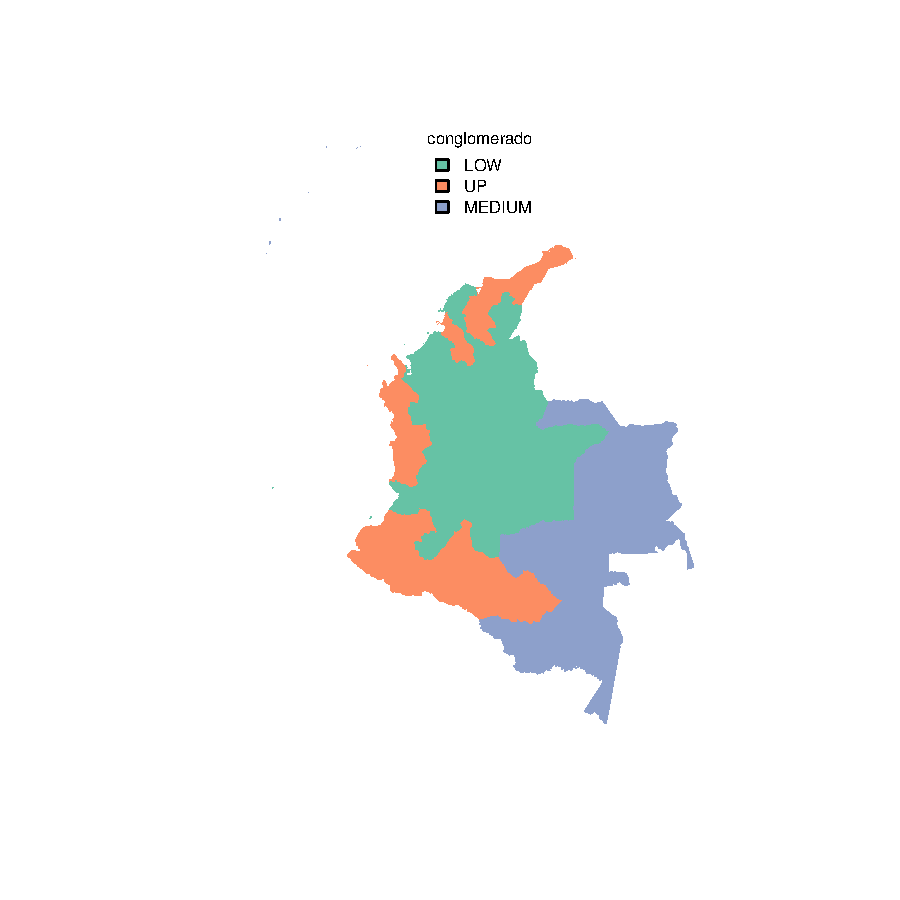
\includegraphics{Proyecto_Final_regresion-plotMapf}
\end{adjustbox}
\caption{Paises conglomerados segun sus indicadores sociopolaticos}\label{clustmap}
\end{figure}

\clearpage

\endinput
